%%% Local Variables: 
%%% mode: latex
%%% TeX-master: "../KanjiHWR"
%%% End: 

\chapter{Japanese Script}
\label{chap:japanasescript}

%xxx - Why this section? 
%xxx   The purpose of this section is 
%xxx   It would be off purpose, if 
%xxx - What goes into this section?
%xxx   The main content of this section is 
%xxx   * if describing a problem: why is the problem relevant.
%xxx   * if describing a solution to a problem: what alternatives were
%xxx     there to solve it, why was this solution chosen? 
%xxx     what made it the best choice? was it the optimal solution?
%xxx - How will this section be structured and organised?
%xxx   The organisational structure of the section 
%xxx - In what style will it be written?
%xxx   The style of writing will be 
%xxx - Next action - what to write first?
%xxx   The next part to write is

The Japanese writing system has a long history. It goes back to around 800 A.D. 
The Japanese script is in fact a writing system, as Japanese is denoted in 
a combination of three different scripts: \emph{Hiragana}, \emph{Katakana} and 
\emph{Kanji}. Kanji is a conceptual script, where each character bears the 
meaning of one or more semantic concepts and represents morphemes. 
Hiragana and Katakana are both syllabic scripts, and the individual characters do
not bear reference to concepts or even words, but merely to phonological units, 
usually two phonemes.

In this chapter, the development of the script will be reviewed in 
section~\ref{sec:ashorthistoryofjapanesewritingsystem}.
In section~\ref{sec:modernjapanesewritingsystem} the current Japanese writing 
system will be exemplified, with a focus on the Kanji in 
section~\ref{sec:compositionofKanji}. Hiragana and Katakana will be reviewed in
section~\ref{sec:kana}, which centres around the Kana scripts. 
Machine processing of the different Japanese scripts and the difficulties that
go along will be demonstrated in section~\ref{sec:machinewritingofjapanese}.
The difficulties of learning to use the Japanese script will be illustrated in 
section~\ref{sec:japanesedifficulties}.

\section{A Short History of the Japanese Script}
\label{sec:ashorthistoryofjapanesewritingsystem}

The historical development of the Japanese script is tightly connected to the 
history of the Kanji characters. Kanji, in Japanese 
\cjk{漢字}~(Jap. pron. \cjk{カンジ} / Kanji; Eng.~lit.~\emph{Han~characters}) 
refers to the 'characters of the Han', meaning the Han Dynasty 
(206 B.C.-220 A.D.; simplified Chinese: \cjk{汉朝}; traditional Chinese: 
\cjk{漢朝}) \shortcite{Foljanty1984}. In Mandarin the same characters are 
referred to as \emph{Hànzì} (simplified Chinese: \cjk{汉字}; 
trad. Chinese: \cjk{漢字}).
Note, that the first character \cjk{漢} (Chin. 'han', Jap. 'kan', Eng. 'Han') 
of both the words \emph{Han dynasty} and \emph{Kanji} is identical in Japanese 
and traditional Chinese, even though it has a different reading in the 
Chinese and Japanese language. In traditional Chinese the character with
the same meaning (\cjk{汉}) has a different shape. This apparent oddity will be 
explained in greater detail in 
section~\ref{sec:historicaldevelopmentofjapanesescript}.

\subsection{Historical Development}
\label{sec:historicaldevelopmentofjapanesescript}
%see \shortcite{Foljanty1984} 2.1.1-2.1.3
%see wikipedia article
%see \shortcite{Grassmuck1997}
%see \shortcite{Chamberlain1982} for the Kojiki

The Kanji script as developed and coined by the Han is in principle still valid 
today. It is used alone or in combination with phonetic spelling in China, Japan,
Taiwan, Hong Kong. In Vietnam it was used before it was replaced with the 
Vietnamese alphabet (Viet.: 'quốc ngữ', Eng. lit. 'national language', Eng. 
'national script'), a script based on the Latin alphabet. In South Korea the Han 
characters were in use until they were replaced with 
Hangul~(Kor. with Han characters \cjk{韓國語}; Eng. 'Korean')~\shortcite{Foljanty1984}.

The Kanji characters were brought to Japan by Koreans living in Japan around 
300-400 A.D. Since the Kanji were used by the Koreans to write 
Hangul they also used it to write Japanese. There was no other Japanese script 
before that time. Reports about an original Japanese script called 
\emph{Jindai Moji} (Jap. \cjk{神代文字}; Eng. 'scripts of the age of the gods')
could not be proved. They are now assumed to be a political and speculative 
invention by Japanese Nationalists in the early 
19th.~century~\shortcite{Foljanty1984}. According to \shortcite{Lange1922}
the \emph{Kogo Shūi} (Jap. \cjk{古語拾遺}; a historical record of the Inbe clan),
which was written around 800 B.C. denies the presence of a Japanese native
script before the introduction of the Han characters. However, the questions
seems irrelevant in the sense, that no longer text or document has been found,
written in that script.

In the Christian year 712 an ancestral act of writing was performed at 
Japanese emperor Temmu's court. Hieda~no~Are, a member of the guild of the 
\emph{Kataribe} or reciters, basically a Japanese Griot, dictates the 
\emph{Kojiki} (Jap. \cjk{古事記}; Eng. 'Record of Ancient Matters') to 
Ō~no~Yasumaro. Ō~no~Yasumaro wrote the Kojiki, which is not the first written 
document found in Japan, however it is Japan's oldest attempt to write down 
spoken Japanese~\shortcite{Grassmuck1997,Chamberlain1982}.

At the time the Han characters were first used to write Japanese, 
they were already a developed script. The script was more than 1,000 years old
since the characters stabilised to their modern form within the Han 
period. %\footnote{Also see time line in section~\ref{sec:app:Kanjitimeline}.}. No timeline available.
The first Chinese characters were found on oracle bones from the Shang Dynasty
(Chinese \cjk{商朝}), which ruled over China some 500 to 600 years within the 
time period between 1600 B.C. and 1046 B.C.~\shortcite{Grassmuck1997,Guo2000}.

According to the Kojiki, a scholar called Wani (Jap. \cjk{王仁}) from Korea 
brought two foundational Chinese books to Japan, the \emph{Lunyu} 
(Simplified Chin. \cjk{论语}; trad. Chinese: \cjk{論語}; Eng. 'Analects'), 
also known as \emph{The Analects of Confucius} and 
the \emph{Qianziwen} (Chin./Jap. \cjk{千字文}; Jap. 
pron.~\cjk{センジブン}/senjibun; Eng. 'The Thousand Character Classic'),
which is a Chinese poem used as a primer for teaching Chinese characters to 
children. It contains exactly one thousand unique 
characters~\shortcite{Grassmuck1997}. However, \shortcite(Lange1922) demurs 
strongly against this view and assumes an evolving adoption of the Kanji in
Japan. This view seems more plausible, since it has been proved that Japan 
had contact to Korea even in the time before common era and had contact to 
China at least from the first century A.D. The Chinese language comprehends more
than 40,000 Hànzì characters lexicographically. Only around 25\% of those 
including about 250 \emph{Kokuji} (Jap. \cjk{国字}; Eng. 'national characters') 
are in Japanese dictionaries. Only around 2,000-3,000 of those are part of the 
common characters~\shortcite{Foljanty1984}. 

The Japanese Ministry of Education issued a list of 1,850 standard Kanji in 1946
under the name of \emph{Tōyō Kanjihyō} (Jap.~\cjk{当用漢字表};
Eng.~'list of Kanji for general use'). The list of Tōyō Kanji was slightly 
revised and extended in 1981 and comprised 1,945 Kanji as the Jōyō Kanji
(Jap. \cjk{常用漢字}; Eng. 'often used Kanji')~\shortcite{Foljanty1984}.
As of 2010 a revised list of 2,131 characters is in official 
use~\shortcite{Noguchi2009}. 

In China there had been a spelling reform in the 1950s, affecting many of the
general use characters, resulting in simplified Chinese. In Japan, the Ministry
of Education issued it's own reform when the Tōyō Kanji list was introduced.
However, the Japanese reform affected a smaller set of characters of only a few 
hundred and resulted in Shinjitai (Jap. shinjitai: \cjk{新字体}; 
Jap. kyūjitai: \cjk{新字體};
Jap. pron. \cjk{シンジタイ}/shinjitai; Eng. 'new character form'), 
which replaced the Kyūjitai 
(Jap. shinjitai: \cjk{旧字体}; Jap. kyūjitai: \cjk{舊字體}; 
Jap. pron.~\cjk{キュウジタイ}/kyūjitai; Eng. lit. 'old character forms'). 
This explains how some characters are still identical in traditional Chinese and 
Japanese, because they were not affected by any spelling reform, like the 
aforementioned \cjk{漢} (Jap. pron. \cjk{カン}/kan; Chin. pron. 'hàn'),
while other characters are different, like the simplified 
Chinese 'hàn': \cjk{汉}. Henceforth, and throughout this document, all Japanese characters are in the new character form shinjitai.

\section{The Modern Japanese Writing System}
\label{sec:modernjapanesewritingsystem}

%see \shortcite{Foljanty1984} 3.1
%see \shortcite{Lange1922} p.64
%see \shortcite{Tsujimura2007} for morphology stuff
%see \shortcite{Grassmuck1997}

The Japanese writing system has a complex structure. The three scripts 
\emph{Hiragana} (section~\ref{sec:hiragana}),
\emph{Katakana} (section~\ref{sec:katakana}) and
\emph{Kanji} (section~\ref{sec:compositionofKanji}),
are combined to one writing system. Each script has its task within the system:
\begin{itemize}

  \item Kanji are used to write lexical morphemes, i.e. content-bearing morphemes.

  \item Katakana are used to transcribe foreign words, borrowings and 
        nonstandard areas.

  \item Hiragana are used to write grammatical morphemes and anything else that
        is not written in one of the other two scripts, e.g. the spoken syllables
        of a word that should be written with a Kanji character unknown to the 
        writer of that word.
\end{itemize}
The actual writing system is mainly based on Kanji and Hiragana, catenated to
Kanji-Kana blended writing.
\begin{exe}
\ex\label{exe:mariaYamada}
\begin{xlist}
\ex \label{exe:mariaYamadaSplit}
\gll 
 \cjk{マリア:} 
 \cjk{山田さん、} 
 \cjk{「火の鳥」} 
 \cjk{という} 
 \cjk{アニメ} 
 \cjk{を} 
 \cjk{もう} 
 \cjk{見ました} 
 \cjk{か。} \\
% Maria: Yamada-San, [kanotori] toiu anime wo mou mimashita ka.\\
 Maria: Yamada-San, [Firebird] say anime \textsc{obj-particle} already seen \textsc{question-particle} \\
\trans 'Maria: Ms Yamada, say, have you seen the Firebird cartoon yet?' \\
Taken from~\shortcite{Katsuki2006Book}
\ex\label{exe:mariaYamadaFull}
 \begin{CJK} 
  マリア:山田さん、「火の鳥」というアニメをもう見ましたか。
 \end{CJK}
\end{xlist}
\end{exe}
In example~(\ref{exe:mariaYamadaSplit}), the blending of the different scripts 
can be seen:\\
Both the foreign name  \cjk{マリア} (Eng. 'Maria') and the borrowing 
\cjk{アニメ} (\emph{anime}, Jap. short for Eng. 'animation') are written in 
Katakana. Kanji are used for:
\begin{itemize}
\item The Japanese name \cjk{山田} (\emph{Yamada}).
\item The nouns \cjk{火}~(Eng. 'fire') and 
      \cjk{鳥}~(Eng. 'bird').
\item The verb stem \cjk{見}~(Eng. 'see').
\end{itemize}
The rest is written in Hiragana:
\begin{itemize}
  \item The politeness ending \cjk{さん}~(\emph{san}; 
        Eng. equiv. 'Mr/Ms/Mrs') for addressing a person with their name.
  \item The genitive particle \cjk{の}~(\emph{no}) between 
        \cjk{火}~(Eng. 'fire') and \cjk{鳥}~(Eng. 'bird'), to yield 
        \cjk{火の鳥}~(Eng. 'Firebird').
  \item The interjection \cjk{とうい}~(Eng. 'say').
  \item The object particle \cjk{を}~(\emph{wo}).
  \item The adverb \cjk{もう}~(Eng. 'already').
  \item The past tense conjugation and politeness ending of the 
        verb \cjk{ました}~(\emph{mashita}).
  \item The question particle \cjk{か}~(\emph{ka}).
\end{itemize}

Three different scripts are used next to each other in one sentence,
indistinguishable for the untrained eye. Example~(\ref{exe:mariaYamadaFull}) 
shows the sentence as it is printed in~\shortcite{Katsuki2006Book}. Without prior
knowledge of the different Japanese scripts it is hard to even distinguish
the individual word tokens, as blanks are usually absent in Japanese writing.
Other than actually knowing the words, which is not the usual case for a 
beginner of learning Japanese, often the change of script is the only way to 
recognise a new token. However, Kanji and Hiragana are often used within the same
word, too.

Despite those complexities, other features of the Japanese writing system are 
simpler than in latin-based alphabetic scrips. 
For example, there is no capitals or lowercase letters.
Each character has a reserved space of roughly the same size.
In the following sections, the different scripts will be presented in greater 
detail. Their composition and use will be discussed.

\subsection{Kana \cjk{かな}}
\label{sec:kana}

If the Japanese had abolished the Chinese characters after formation of the
syllabic scripts and used only those, studying the Japanese script would be
a less complex task. \shortcite{Lange1922} reports about attempts to remove
the Kanji from Japanese and use the Kana or even Latin script, so called
\cjk{ロマジ} (\emph{Romaji}, a Latin or 'Roman' transcription of Japanese; 
Eng. lit. 'Roman characters'). 
However, non of those attempts succeeded and both Kana scripts serve as 
auxiliary scripts to the predominant Kanji characters. 

The Chinese characters have been used in two ways in Japanese. 
Firstly, in order to express the morphological content of a character,
but also in order to use the sound of the character as a syllable.
The characters that have been used as syllables were transformed to two 
separate short-hand notations. 
One way used cursive writing of the sound Kanji, reducing the character 
graphically, such that its original shape became virtually in-cognisable.
This development resulted in the Hiragana script. An example of that kind of 
reduction is shown in figure~\ref{fig:reductiontohiragana}.
\begin{figure}[htbp]
\begin{center}
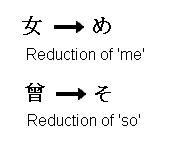
\includegraphics[scale=0.7]{images/reductiontohiragana.png}
\caption{Reduction from Kanji to Hiragana}
\label{fig:reductiontohiragana}
\end{center}
\end{figure}
The other method of reduction uses only one of the character's Graphemes in
order to represent the whole character. That reduction process (see 
figure~\ref{fig:reductiontokatakana}) lead to the development of the
Katakana script.
\begin{figure}[htbp] 
\begin{center}
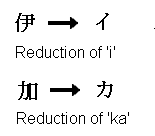
\includegraphics[scale=0.7]{images/reductiontokatakana.png}
\caption{Reduction from Kanji to Katakana}
\label{fig:reductiontokatakana}
\end{center}
\end{figure}

Using cursive or reduced characters became popular in the 9th century already.
Both Hiragana ('smoothened Kana') and Katakana ('fragmented Kana') can easily be 
distinguished from the more complex Kanji. They represent a different linguistic 
content than the Kanji, namely rather a syllable than a morpheme.
The fact that two parallel scripts came into existence can be explained by 
their use of different social groups. Hiragana are a product of the literately 
active court ladies, while Katakana were developed in the Buddhist seminaries.
The current system knows 46 Hiragana and Katakana for identical 
syllables~\shortcite{Foljanty1984}. See appendix~\ref{sec:app:kana} for a 
complete list of characters.

\subsubsection{Hiragana \cjk{ひらがな}}
\label{sec:hiragana}

Hiragana is one of the three syllabic scripts. The third one, 
\emph{Hentaigana} can be neglected, as it is not in active use any more. %xxx citation missing here
In principle each character represents a syllable, which can contain either a 
vowel (like 'u', \cjk{う}), a consonant and a vowel (like 'ta', \cjk{た}) or the 
nasal consonant \cjk{ん} ('n').
Hiragana are used for any words for which no Kanji exist, like 
\cjk{から}~(\emph{kara}, Eng. 'from') or grammatical particles like the object 
particle \cjk{を} (\emph{wo}, works like a case marker).
Additionally, Hiragana are used, when the Kanji is not known to the writer or 
reader~\shortcite{Foljanty1984}. 

For instance, a writer may even passively know a Kanji, but not be able
to actively produce it. Say the Kanji in question was \cjk{新}~(Jap. pron. 
atara/\cjk{あたら} and shin/\cjk{シン}; Eng. 'new'). Example~(\ref{exe:newKanji})
shows first the spelling with the Kanji character 
in~(\ref{exe:newKanjispelling}), where the Hiragana parts are underlined.
Then the alternative spelling without the Kanji character 
in~(\ref{exe:newhiraganaspelling}) (with blanks in between, in order to visualise
the individual characters and their readings). The underlined last part is 
identical, just the Kanji character has been replaced with an alternative 
Hiragana spelling.
\begin{exe}
\ex \label{exe:newKanji}
\begin{xlist}
\ex \label{exe:newKanjispelling}
\gll \cjk{新}\underline{\cjk{しい}} \\
atara\underline{shii} \\
\trans 'new'

\ex \label{exe:newhiraganaspelling}
\gll \cjk{あ} \cjk{た} \cjk{ら} \underline{\cjk{し}} \underline{\cjk{い}} \\
a ta ra \underline{shi} \underline{i} \\
\trans 'new'
%新聞
%しんぶん
\end{xlist}
\end{exe}

Hiragana can be modified with
\begin{itemize}

  \item \textbf{Dakuten} (\cjk{濁点}, Jap. pron. \cjk{ダクテン}/dakuten;
        Eng. 'turbid'; Jap. coll. \emph{ten-ten}, Eng. 'dot dot') for 
        syllables with a voiced consonant phoneme. The dakuten glyph (\cjk{゛})  
        resembles a quotation mark and is directly attached to a 
        character~\shortcite{Foljanty1984}.

  \item \textbf{Handakuten} (\cjk{半濁点},
        Jap. pron. \cjk{ハンダクテン}/handakuten; 
        Eng. 'half-turbid'; Jap. coll. \emph{maru}, Eng. 'circle') for syllables 
        with a /p/ morpheme. The glyph for a 'maru' is a little circle (\cjk{゜})
        that is directly attached to a character~\shortcite{Foljanty1984}.

\end{itemize}
\begin{exe}
\ex \label{exe:dakuten}
\begin{xlist}
\ex \label{exe:standarddakuten}
\gll \cjk{た} $\rightarrow$ \cjk{だ}, \cjk{き} $\rightarrow$ \cjk{ぎ}, \cjk{ふ} $\rightarrow$ \cjk{ぶ}, \cjk{へ} $\rightarrow$ \cjk{べ}, \cjk{そ} $\rightarrow$ \cjk{ぞ} \\
ta $\rightarrow$ da, ki $\rightarrow$ gi, fu $\rightarrow$ bu, he $\rightarrow$ be, so $\rightarrow$ zo \\

\ex \label{exe:handakuten}
\gll \cjk{は} $\rightarrow$ \cjk{ぱ}, \cjk{ひ} $\rightarrow$ \cjk{ぴ}, \cjk{ふ} $\rightarrow$ \cjk{ぷ}, \cjk{へ} $\rightarrow$ \cjk{ぺ}, \cjk{ほ} $\rightarrow$ \cjk{ぽ} \\
ha $\rightarrow$ pa, hi $\rightarrow$ pi, fu $\rightarrow$ pu, he $\rightarrow$ pe, ho $\rightarrow$ po \\
\end{xlist}
\end{exe}
Example~(\ref{exe:dakuten}) shows the dakuten in use. 
In~(\ref{exe:standarddakuten}) the turbidity, i.e. the transformation from a 
fortis to a lenis consonant is exemplified. 
The dakuten can only be applied to characters that begin with the sounds 
/k/, /s/, /t/ and /h/. For the consonants 'k', 's' and 't' this is natural in the
way that the place of articulation remains the same for the consonants 'g', 'z' 
and 'd' and their corresponding sounds /g/, /z/, /d/, 
compared to /k/, /s/ and /t/.
Assuming the place of articulation, a changed intensity and use or no use of the 
vocal cords as the natural connection between the characters with and without 
a \emph{ten-ten}, there is a difference for the sound /b/:\\
Since there is no Hiragana character to match a /p/ sound, the characters with
an /h/ sound serve as a basis to form the modified characters with a /b/ sound.
Quite logically, since the Handakuten only yields a /p/ sound, the same set of
characters, namely, the 'h'-row in the Hiragana character set, is modified in 
order to obtain the 'p'-row. In~(\ref{exe:handakuten}) the transformations from 
the /h/ and /f/ sounds to /p/ are shown in a complete list\footnote{
%xxx citation missing - this is my very own assumption. plausible, but true?!
The /f/ sound in Japanese is 'lighter' than in English. Concretely, the place of
articulation for /f/ in English is labio-dental, whereas in Japanese it is 
virtually bi-labial. Therefore, the phonation stream creates less friction and
the allophone of the /f/ phoneme that is typical for the Japanese language sounds
similar to an /h/ sound.}.

\subsubsection{Katakana \cjk{カタカナ}}
\label{sec:katakana}

Just like the Hiragana, the Katakana form a syllabic script. They are mainly used
to transcribe foreign words like names and borrowings, like \cjk{マリア}
(\emph{maria}) and \cjk{アニメ} (\emph{anime}) from 
example~(\ref{exe:mariaYamada}). Another use of the Katakana is called 
\emph{Furigana}, little notations next to Kanji in order to indicate their 
reading. They were developed around the period of the Heian, from 
\emph{Manyogana}, Kanji characters that were used to denote pronunciation.
For example the character \cjk{加}, which was used to represent the pronunciation
\emph{ka}, was shortened to \cjk{カ}, by leaving out the second part 
\cjk{口}~\shortcite{Hadamitzky1995}. Compare also figure~\ref{fig:reductiontokatakana}. For a full table of Katakana characters see 
appendix~\ref{sec:app:katakana}. The dakuten can be applied to Katakana as well 
and have the same meaning.
%xxx maybe some more about katakana here, of required. probably not.

\subsection{Composition of the Kanji \cjk{漢字}}
\label{sec:compositionofKanji}

\subsubsection{Typology}
\label{sec:typologyoftheKanji}

In order to study the Kanji and their composition, it is useful to know how they
were first indented and built. Integrated as the integral part into the Japanese
writing system, despite the reform and the choice different subsets of what is 
considered the standard character set, the characters are still mainly composed
the way as intended by the scholars of the Han period.

From the religious writings on the oracle bones mentioned in 
section~\ref{sec:historicaldevelopmentofjapanesescript} a secular script 
emerged. In parallel, the process of graphical abstraction advanced and
finished around 100-200 A.D., leaving aside the modern reforms of the 
20th~century. The invention of the paint-brush around 100 B.C. improved and 
simplified writing, also the writing surfaces in their order of appearance,
bone, stone, metal, wood and then paper, brought further simplification and
spreading of writing. Paper and paint-brush offered the possibility to write
without hindrance and technical coincidences, therefore it was possible to
standardise the characters and improve them from artistic and aesthetic 
viewpoints.

%xxx: Put some real Kanji pictograms here after Kano1990 lesson 1+2
\begin{figure}[htbp]
\includegraphics[scale=0.5]{images/Kanjipictograms.png}
\caption{Kanji pictograms}
\label{fig:Kanjipictograms}
\end{figure}

\begin{table}[htbp]
  \begin{tabular}{| l l l l|}
    \hline
    Radical 1 & Radical 2 & Result & Meaning \\
    \hline
    \cjk{日} ('sun') & \cjk{月} ('moon') & \cjk{明} ('bright') & both the sun and the moon are 'bright' \\
    \hline
    \cjk{人} ('man') & \cjk{木} ('tree') & \cjk{休} ('rest') & a man is 'resting' beside a tree \\
    \hline
    \cjk{田} ('rice field') & \cjk{力} ('power') & \cjk{男} ('man, male') & 'a man' is powerful on the rice field \\
    \hline
    \cjk{女} ('woman') & \cjk{子} ('child') & \cjk{好} ('love') & a woman 'loves' a child \\
    \hline
    \cjk{木} ('tree') & \cjk{木} ('tree') & \cjk{林} ('wood, grove') & two trees make a 'wood' \\
    \hline
    \cjk{木} ('tree') & \cjk{林} ('wood') & \cjk{森} ('forest') & three trees form a 'forest' \\ 
    \hline
    \cjk{門} ('gate') & \cjk{日} ('sun') & \cjk{間} ('between') & the sun can be seen 'between' the doors of the gate \\
    \hline
  \end{tabular}
\caption{Kanji ideograms}
\label{table:Kanjiideograms}
\end{table}

\begin{table}[htbp]
  \begin{tabular}{| l c l |}
    \hline
    Class radical & Sound radical /ki/ & meaning \\
    \hline
    \cjk{土} ('earth') & \cjk{奇} & \cjk{埼} 'spit, promontory, cape' \\
    \cjk{山} ('mountain') & \cjk{奇} & \cjk{崎} 'promontory, cape, spit' \\
    \cjk{石} ('stone') & \cjk{奇} & \cjk{碕} 'cape, promontory, spit' \\
    \cjk{王} ('jade') & \cjk{奇} & \cjk{琦} 'gem, precious stone' \\
    \cjk{糸} ('thread') & \cjk{奇} & \cjk{綺} 'figured cloth, beautiful' \\
    \cjk{馬} ('horse') & \cjk{奇} & \cjk{騎} 'riding on horses' \\
    \cjk{宀} ('roof') & \cjk{奇} & \cjk{寄} 'to gather' \\
    \cjk{金} ('metal') & \cjk{奇} & \cjk{錡} 'cauldron, chisel' (Chinese only) \\
    \hline
  \end{tabular}
\caption{Kanji phonograms}
\label{table:kicombinations}
\end{table}

The Kanji can be classified according to their building principle:
\begin{enumerate}
 \item \textbf{Pictograms} are graphically simplified images of real artefacts.
       The examples in figure~\ref{fig:Kanjipictograms} 
       after~\shortciteANP{Kano1990}~\citeyear{Kano1990} show the graphical 
       reduction process. Pictograms are only a small minority among the Kanji,
       their number ranges around 120. Another 100 pictograms appear as a part of
       more complex characters~\shortcite{Foljanty1984}.
       
 \item \textbf{Ideograms} are combinations of two or more pictographical
       characters. They often bear a more abstract meaning than a simple 
       pictogram. The abstract meaning of the complex character is meant to be 
       associated with the content of the individual parts. The number of 
       ideograms is fairly small, too. Abstract terms like 
       'top' (Jap.~\cjk{上}, pron. \cjk{うえ}/ue), 
       'bottom' (Jap.~\cjk{下}, pron. \cjk{した}/shita),
       'left' (Jap.~\cjk{左}, pron. \cjk{ひだり}/hidari),
       'right' (Jap.~\cjk{右}, pron. \cjk{みぎ}/migi)
       and numbers like
       'one' (Jap.~\cjk{一}, pron. \cjk{いち}/ichi),
       'two' (Jap.~\cjk{二}, pron. \cjk{に}/ni),
       'three' (Jap.~\cjk{三}, pron. \cjk{さん}/san),
       'four' (Jap.~\cjk{四}, pron. \cjk{し}/shi),
       'five' (Jap.~\cjk{五}, pron. \cjk{ご}/go)
       and so forth can be regarded as parts of the 
       ideograms~\shortcite{Foljanty1984}.
       See table~\ref{table:Kanjiideograms} (after \shortcite{Kano1990}) for 
       some examples on Kanji pictograms.

 \item \textbf{Phonograms} are combinations of two Kanji characters. One of those
       refers to a concept class (for \emph{class characters} or \emph{radicals},
       see section~\ref{sec:radicals}), 
       while the other character exclusively bears a phonetic value. The content
       of the second part of a phonogram is not relevant and can be ignored.

       In table~\ref{table:kicombinations} the character 
       \cjk{奇} (Jap. pron. \cjk{き}/ki, Eng. 'strange') is used for the purpose
       of pronunciation only (/ki/), while the radical defines an
       object class. Object classes can be categories like 'human and human 
       actions', 'metal', 'horse', 'roof / under a roof' etc.
       The semantic identity within the \emph{Morphogram} is assembled with two
       reference figures. The pronunciation part is identical for all characters,
       it serves as a selection criterion within a semantic class selected by 
       the class radical~\shortcite{Foljanty1984}.

\end{enumerate}

As a character type, phonograms are predominant among the Hànzì. Therefore, the
phonogram concept, including the radical concept, was transferred to all Chinese 
characters. Pictograms that are class radicals themselves, are interpreted as 
characters with an empty sound radical. As the phonograms are historically the 
last development step of the Han characters, they constitute a different quality 
in the Chinese script. Phonograms mark the transition between a non-linguistic
pictographic script that does not represent linguistic units, but rather images 
of objects, to a linguistic script. In principle, there is no difference to
an alphabetical or syllabic script. Except, morphemes are represented instead of 
phonemes or syllables. However, one character often denotes more than one 
morpheme~\shortcite{Foljanty1984}.

In Japanese, basically the same relation between the Kanji characters and 
morphemes can be observed. However, the correspondence between the morphemes and 
the syllables (and thus the characters and syllables) is often missing.
Since Chinese has a monosyllabic morpheme structure, a one-to-one correspondence
between morpheme, character and syllable can be observed.
Congruence of character, morpheme and syllable in Japanese can only be found for
Chinese borrowings, but not all of them. The original Japanese vocabulary has
multisyllabic morphemes, therefore some impreciseness arises in the graphical
reproduction of the morpheme structure~\shortcite{Foljanty1984}.

%\subsubsection{Graphemic Elements}
%\label{sec:graphemicelements}

%xxx: see \shortcite{Foljanty1984} 2.1.4.2
%xxx do wee need anything about graphemic elements?

\subsubsection{Radicals}
\label{sec:radicals}

%xxx: see \url{http://japanese.about.com/library/weekly/aa070101a.htm} : radicals
%xxx: see \shortcite{Foljanty1984} 2.1.5 and 2.1.4
%xxx: see \shortcite{Lange1922} p.85ff p.94ff

In section~\ref{sec:typologyoftheKanji} the function of the class characters or
Radicals has been mentioned. The Radicals usually derive from pictograms. The
Chinese systematics with 214 Radicals is used in Japan, as well. Among the 
1945 Jōyō Kanji, only around 50\% of the 214 Radicals is in autonomous use.
22 of them denominate empty classes, 46 denominate classes of only one Kanji.
The Radicals are grouped according to their graphical position inside a Kanji.
Figure~\ref{fig:radicalPositions} shows the groupings of the Radicals 
after~\shortcite{Foljanty1984}.
\begin{figure}[htbp]
\begin{center}
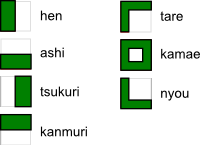
\includegraphics{images/radicalStructure/radicalPositions.png}
\caption{Radical positions in Kanji characters}
\label{fig:radicalPositions}
\end{center}
\end{figure}
The groupings of the Radicals account for a preference of certain Radicals
to appear in a certain category. The selection of the class Radical is primarily
based on semantic criteria. For example, the character \cjk{杉}~(Jap. pron. 
\cjk{スギ}/sugi; Eng. 'cedar') both graphemes have the ability to serve as a 
class Radical. Therefore there is a choice of using either the Radical 
\cjk{木}~(Jap. pron. \cjk{キ}/ki; Eng. 'tree') in the \emph{hen} position, 
or the Radical \cjk{彡}~(Jap. pron. \cjk{カミカザリ}/kamikazari; 
Eng. 'hair ornament') in the \emph{tsukuri} position (see 
Figure~\ref{fig:radicalPositions}). This is very pictographic, since the leaves
of a cedar are long and thin, (see figure~\ref{fig:cedarleaves}), 
therefore the character is most likely an ideogram.
\begin{figure}[htbp]
\begin{center}
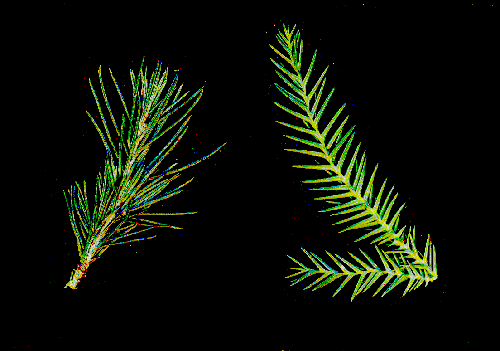
\includegraphics[scale=0.4]{images/radicalStructure/cedar.png}
\caption{Cedar leaves}
\label{fig:cedarleaves}
\end{center}
\end{figure}
Now, the categorisation is purely a semantic choice. The cedar has certainly more
qualities of a tree than qualities of hair, therefore, the class radical is
\cjk{木} (tree) and not \cjk{彡} (hair). \shortcite{Hadamitzky1995} files it 
under the \cjk{木} (tree) class Radical. %Namely at entry 1872

%xxx do we need to say any more about radicals?

\subsubsection{Readings}
\label{sec:readings}

Each character has at least one reading. The Kanji script, being a morphemic 
script does not have a correspondence from character to spoken sound in speech,
like alphabetic scripts. Certainly, alphabetic scripts are often far from a 
one-to-one correspondence between sound and letter, however, the Kanji have 
their very own ways. There are two main readings of the Kanji: \\ 
\begin{itemize}
  \item \emph{On'yomi} (\cjk{音読み}, Jap. pron. \cjk{オンヨミ}/onyomi; 
        Eng. 'sound reading'), which roughly based on its original Chinese 
        reading.

  \item \emph{Kun'yomi} (\cjk{訓読み}, Jap. pron. \cjk{クンヨミ}/kunyomi; 
        Eng. 'concept reading, native reading'), which represents the original 
        Japanese word that happens to be written with a Chinese character. 
        The Kun'yomi are further classified into different types of readings.
\end{itemize}
Because of this, the Kanji that have been developed in Japan only have a 
Kun-reading. A bit more than half of the official Jōyō-Kanji (999 of 1945)
have two readings.
The Japanese Kun-reading was part of the adaption process to the Han-characters,
where the character was taken for its meaning and underlaid with the Japanese
word. The Sino-Japanese reading originated from Chinese borrowings. The 
complex Chinese pronunciation, however, was adapted to the Japanese 
phoneme inventory.

Take for example the Kanji \cjk{山}~(Eng. 'mountain'). 
The original Japanese word for \emph{mountain} is \emph{yama} (\cjk{やま}),
therefore the character \cjk{山} has this reading attached as a Kun-reading.
The Chinese borrowing is \emph{san} (\cjk{サン}), with the meaning 
\emph{mountain}. The reading that is used depends on the 
context~\shortcite{Foljanty1984}.
\cjk{山} is read Sino-Japanese \emph{san} or in a phonetic assimilation \emph{zan} in:
\begin{itemize}
  \item \cjk{山水}, Jap. pron. \cjk{サンスイ}/\textbf{san}sui, Eng. 'landscape'
  \item \cjk{火山}, Jap. pron. \cjk{カザン}/ka\textbf{zan}, Eng. 'volcano'
  \item \cjk{下山}, Jap. pron. \cjk{ゲザン}/ge\textbf{zan}, Eng. 'descent'
  \item \cjk{富士山}, Jap. pron. \cjk{フジサン}/fuji\textbf{san}, Eng. 
        'Mount Fuji'\footnote{'Mount Fuji' is often called 'Fujiyama' in 
        several languages. Thus, the Kun-reading \emph{yama} of \cjk{山} has 
        emerged as a borrowing into other languages, even though in Japan 
        the On-reading is used in the particular case of 'Fuji san'.}
\end{itemize}
\cjk{山} is read in the Japanese Kun-reading in:
\begin{itemize}
  \item \cjk{小山}, Jap. pron. \cjk{コヤマ}/ko\textbf{yama}, Eng. 'hill'
  \item \cjk{山山}, Jap. pron. \cjk{ヤマヤマ}/\textbf{yamayama}, Eng. 'mountains'
\end{itemize}
\shortcite{Hadamitzky1995}

\subsection{Structure of the Japanese Writing System}
\label{sec:structureofwritingsystem}

Having demonstrated the Hiragana in~\ref{sec:hiragana}, the Katakana 
in~\ref{sec:katakana} and the Kanji in section~\ref{sec:compositionofKanji}, 
it is now possible to report about the structure of the writing system as such.
It now becomes apparent, why a sentence like the one presented in 
example~(\ref{exe:mariaYamada}) in section~\ref{sec:modernjapanesewritingsystem} 
is written and spelt the way it is.
\begin{exe}
\ex\label{exe:okurigana}
\gll 
 \cjk{帰りたくない} \\
 kaeritakunai \\
 go-home-want-not \\
\trans 'I do not want to go home' \\
\end{exe}
An important part of the blended writing in Japanese are the 
\emph{Okurigana} (\cjk{送り仮名}, Jap. pron. \cjk{ オクリガナ}/okurigana; 
Eng. 'accompanying characters'). Okurigana are Kana that form 
a word together with a Kanji character~\shortcite{Lange1922}.
For instance, the word in example~(\ref{exe:okurigana}) has only one Kanji 
character: \cjk{帰} (Jap. pron. \cjk{カエ}/kae; Eng. 'go-home'), while the other characters are all Kana characters, that are part of the same word and modify
the verb.
\begin{itemize}
  \item \cjk{り} (\emph{ri}): Flexion of the verb used for \emph{tai}
  \item \cjk{たく} (\emph{taku}): derivation of \emph{tai} = want
  \item \cjk{ない} (\emph{nai}): Negation ending
\end{itemize}
Knowing the two syllabic scripts by heart helps distinguish the Kanji from them.
Therefore it is possible to use the three scripts next to each other, even 
without blanks. The Okurigana further help distinguish different versions of 
the same Kanji, as they sometimes even partially describe the sounds of a 
verb stem.
\begin{exe}
\ex\label{exe:stemspelling}
\begin{xlist}
\ex\label{exe:stemspellingkaeru}
\gll 
 \cjk{変ーえる} \\
 ka-eru \\
 change \\
\trans 'to change something' (transitive) \\

\ex\label{exe:stemspellingkawaru}
\gll 
 \cjk{変ーわる} \\
 ka-waru \\
 change \\
\trans 'to change oneself' (reflexive) \\
\end{xlist}
\end{exe}
Compare for example~(\ref{exe:stemspellingkaeru}) 
and~(\ref{exe:stemspellingkawaru}). 
The Japanese verb ending is 
\cjk{る}~(Hiragana: \emph{ru}). A part of the verb stem are expressed with
Hiragana, too. In~(\ref{exe:stemspellingkaeru}) it is the 
\cjk{え}~(Hiragana: \emph{e}) while in~(\ref{exe:stemspellingkawaru}) it is the 
\cjk{わ}~(Hiragana: \emph{wa}).
The Kanji are further used to write nouns, the Hiragana are used for particles 
and other grammatical functions, while the Katakana are used for foreign words.

%xxx see Foljanty 2.2. kana intro, for this intro - how to write a different language with chinese characters.
%xxx: see \shortcite{Foljanty1984} 3.1-3.2
%xxx wird das nach einleitung ueberhaupt noch gebraucht?

\subsection{Machine Writing of Japanese}
\label{sec:machinewritingofjapanese}

Machine processing of the Japanese scripts has been an issue, ever since humans
started to automate their writing. 
~\shortciteANP{Lange1922}~\citeyear{Lange1922} reports in the foreword to the 
first edition (1896) of his work about difficulties during the printing process. 
Firstly, there was only one printing office in Germany that was able to print 
these kind of things at all. Also, there were technical issues, 
like incompatible letter size and missing characters among the letters 
available. The manufacturing of the appropriate letters delayed the publication.
\begin{quote}
Bei der Drucklegung des Werkes in der Reichsdruckerei, der einzigen Druckerei 
in Deutschland, welche dergleichen zu drucken im stande ist, stellten sich 
leider einige Übelstände heraus. Einerseits sind die Kana-Zeichen, 
welche dieselbe besitzt, zu gross, um als erklärende Zeichen bequem neben die 
chinesischen Zeichen gesetzt werden zu können, andererseits fehlten unter den 
10000 chinesischen Zeichen, die aus Shanghai gekommen, eine Anzahl in Japan 
ganz gebräuchlicher Zeichen. 
Diese mussten entweder aus den vorhandenen Teilzeichen,
die eine andere Form als die übrigen Typen haben, zusammengesetzt werden oder 
sie mussten erst geschnitten werden; 
haupsächlich durch den letzteren Umstand hat sich die Fertigstellung des Werkes 
verzögert.
\end{quote}

\begin{quote}
When the work was printed in the Reichsdruckerei, the only print shop
in Germany capable of printing this kind of work, some mischiefs became obvious.
On one hand, the Kana characters that the Reichsdruckerei had were to large to
be put next to the Chinese characters as explanatory characters, on the other
hand some characters that are very common in Japan were missing among 
the 10000 Chinese characters that came from Shanghai.
The missing characters had to be composed from the partial characters that
had a different shape then the other types, others had to be manufactured.
Mainly because of the last-mentioned circumstances the completion of the
act has been decelerated.
\end{quote}
This quote from \shortciteANP{Lange1922} shows the difficulties an author
was facing when trying to print a book. 
Difficulties in machine writing Japanese also occurred at later stages. The 
technical and practical problems remain to this day, because of the great number
of characters. \shortcite{Foljanty1984} reports that in Japan the number of 
machines needed to print Japanese characters was small, because even business
correspondence was mainly done by hand up to the 1970is. Computers worked with
Katakana only. There were devices like mechanical-type Japanese typewriters,
with around 2000 keys for the different Kanji. A Kanji synthesis system worked
with the internal structure of the Kanji. The 'multi-radical lookup' in 
\shortciteANP{Breen2004}'s \citeyear{Breen2004} system \emph{WWWJDIC} has
a similar concept. A user chooses a number of Radicals from a list and the 
system computes all Kanji that contain these Radicals.
%xxx: sehr stark hier fuer mehr Geschichte: see \shortcite{Grassmuck1997}
In order to handle word processing the Industry standard are Input Method Editors
that come with the operating system. Input Method Editors (IME) use 
Romaji, the Latin transcription of Japanese and a language model in order to
generate a Kanji list, appropriate to the spelling of a 
word. That is necessary since one Kanji can have several readings and Japanese
is rich in homophones~\shortcite{Yuan2005,Hadamitzky1995}. 
Certainly the most modern input method for Japanese characters is handwriting
recognition. The difficulties of other input methods show that there is 
great need for a better and faster method of input. See 
section~\ref{sec:hwrofhanziandKanji} for a description of research 
efforts in order to provide technology for using handwriting as an input method 
for Japanese.

\section{Difficulties of the Japanese Script for Learners}
\label{sec:japanesedifficulties}

%xxx different readings
%Heisig has developed a method to learn the Kanji.
%the%several other methods exist

There are at least four ways to learn the Japanese Script. 
With \emph{learning the Japanese script} we mean \emph{learning the Kanji}.
For the Hiragana and Katakana are only small sets of syllabic characters,
the effort to study those is only slightly larger than learning the Latin 
alphabet. The number of different learning methods and the diversity of advice
that can be found on this topic on the Internet and in teaching books suggests
that learning the Kanji is regarded a difficult issue.
It is apparent that the difficulties lie in the complexity of the Kanji, 
but also on the structure of the writing system as such. 
\shortciteANP{Stahlmann2004}~\citeyear{Stahlmann2004} reports the subjective 
impression of many learners that Chinese is among the most challenging languages
and even seems daunting. Japanese is no different, as most of the difficulties 
of the Chinese language are characteristics of Japanese as well. 
The pronunciation of Japanese is comparatively simple for a European learner, 
as the phonetic inventory of the language is similar to that of 
English~\shortcite{Tsujimura2007}. On the other hand, the Japanese writing 
system with its three different scripts and several readings of a character 
has other interweavements as demonstrated in the previous sections.
Despite the difficulties, the interest in the Japanese language and 
culture is unbowed:\\
There are many books available centred around cultural interchange between
the western and Japanese culture. For example,~\shortcite{Haschke2008} present
German words of Japanese heritage, i.e. a miniature etymological lexicon.
The sheer existence of that type of book on the free market suggests that 
Japanese language and culture radiate fascination into the western world.
Therefore, there is a great need for learning methods.

The four groups of learning methods are:
\begin{enumerate}
  \item \textbf{Writing Repetition} - Each Kanji has to be written several times
        until its meaning and the readings are full known to the learner.
        Most Kanji books generally follow this concept.

  \item \textbf{Flash Cards} - Instead of writing the Kanji, the flash card 
        method teaches the passive knowledge. Flash cards for Kanji are readily
        available and can be home made easily.

  \item \textbf{Mnemonic methods} - Methods that use mnemonics in order to help
        a learner memorise the Kanji.
        \begin{enumerate}
          \item \textbf{Textual mnemonics} The \emph{Heisig method} assigns a 
                unique mnemonic to each Kanji in order make it more memorable. 
                These mnemonics are little stories oriented toward the shape
                of a Kanji and do not necessarily have a connection to the 
                actual meaning of a Kanji. They are just mnemonics. 
                The Heisig method is a two-part method. In the first part
                the learner studies all the Kanji and their translations, 
                in the second part the Japanese readings are 
                introduced~\shortcite{Heisig2007}.

          \item \textbf{Visual mnemonics} \emph{Kanji Pict-O-Graphix} is 
                another mnemonic method. In this method the Kanji are 
                depicted with images that represent the meaning of the Kanji.
                The stories are therefore more visualised than in the Heisig 
                method~\shortcite{Rowley1992}.
          \end{enumerate}
\end{enumerate}


\subsection{Learner's Problems}
\label{sec:learnersproblems}

\begin{enumerate}
  \item \textbf{Similar Kanji.} In order to be able to distinguish characters 
        like \cjk{営} in \cjk{営業} and \cjk{管} in \cjk{管理} a high level of
        concentration is necessary. Especially, when Japanese is mostly written
        on the computer and not by hand, the muscular memory 
        does not help any more. Therefore the more Kanji are known, the more 
        difficult it becomes to distinguish similar Kanji.

  \item \textbf{Compounds.} Often, new vocabulary is studied, rather than new 
        Kanji. The vocabulary are often composed of Kanji characters that are 
        already known. Studying time is needed in order to study the vocabulary 
        and compounds. Therefore it is difficult to study new Kanji at the same
        time.

  \item \textbf{Unusual readings.} Since Kanji have several readings, 
        it is useful for a learner to study the most frequent ones.
        For example, the Kanji \cjk{雪}~(Eng. 'snow') has two 
        standard readings (see section~\ref{sec:readings} for more on 
        readings):\\
        The Chinese reading (\emph{on-reading}) is \cjk{セツ}/setsu, 
        while the Japanese reading (\emph{kun-reading}) is \cjk{ゆき}/yuki.
        These two readings occur in very usual Japanese words, having a 
        relation to \emph{snow}. \emph{Setsu} occurs in
        \cjk{雪害}~(Jap. reading \cjk{セツガイ}/\emph{setsu}gai; 
        Eng. 'damage through snow') and
        \cjk{新雪}~(Jap. reading \cjk{シンセツ}/shin\emph{setsu}; 
        Eng. 'fresh snow').
        \emph{Yuki} occurs in
        \cjk{初雪}~(Jap. reading \cjk{ハツユキ}/hatsu\emph{yuki}; 
        Eng. 'first snow of the season'),
        \cjk{大雪}~(Jap. reading \cjk{オウユキ}/ou\emph{yuki}; 
        Eng. 'heavy snow') and
        \cjk{雪合戦}~(Jap. reading \cjk{ユキガッセン}/\emph{yuki}gassen; 
        Eng. 'snowball fight'). 
        Similarly, the Kanji \cjk{崩}~(Eng. 'break down, destroy') 
        has two standard readings:\\
        The Chinese reading (\emph{on-reading}) is \cjk{ホウ}/hou, 
        while the Japanese reading (\emph{kun-reading}) is \cjk{くず}/kuzu.
        The Kanji \cjk{崩} in the reading \emph{kuzu} does not appear as an 
        individual word, in the following examples it is used as a 
        verb stem only. These two readings occur in Japanese words related to 
        \emph{break down}. \emph{Hou} occurs in 
        \cjk{崩御}~(Jap. reading \cjk{ホウギョ}/\emph{hou}gyo; 
        Eng. 'death of the emperor').
        \emph{Kuzu} occurs in 
        \cjk{山崩れ}~(Jap. reading \cjk{ヤマクズレ}/yama\emph{kuzu}re; 
        Eng. 'landslide') and 
        \cjk{切り崩す}~(Jap. reading \cjk{キリクズス}/kiri\emph{kuzu}su; 
        Eng. 'erode').
        The compound of the two, forms a logical unit 
        \cjk{雪崩}~(Eng. 'avalanche', which could be described semantically as a 
        *'snow landslide'). The reading however, is quite unexpected. Instead of
        a combination of 'yuki' and 'kuzu(re)' to yield *\emph{yukikuzure},
        the correct reading is \emph{nadare}~(Jap. \cjk{ナダレ}).
        Unexpected readings like that can be a frustrating and exhausting 
        experience for a learner. % Kanji 949 and 1122
        The reading \emph{nadare} in this example is a \emph{Jukujikun}.
        Jukujikun~(Jap. \cjk{熟字訓}; pron. \cjk{ジュクジクン}/jukujikun; 
        Eng. 'compound kun readings') are specialised Kun-readings that only 
        occur in fixed compounds, comparable to \emph{irregular} words in 
        English~\shortcite{Wydell1998}.
     
  \item \textbf{Alternative Kanji.} Some Kanji have the same meaning and reading,
        yet look differently. For instance the number \emph{one} can be written
        \cjk{壱} or simply \cjk{一}.

  \item \textbf{Homophones.} Japanese has several homophones. An extreme example
        is \cjk{きょう}~(\emph{kyou}): Around 80 Kanji have at least an 
        alternative reading \emph{kyou}. 
        Also, for example, there are three Kanji 
        that can be read \cjk{アツイ}/atsui,namely, 
        \cjk{熱い}~(Eng. 'hot' - for objects or feelings), 
        \cjk{暑い}~(Eng. 'hot' - for the weather) and 
        \cjk{厚い}~(Eng. 'thick' - for clothes; 'kind, warm' - as a 
        characteristic of a person). This can be confusing for a learner.

  \item \textbf{Infrequent Jōyō Kanji.} There are Kanji that are in the official
        list of daily use Kanji, but in fact they are actually not frequently 
        used. These can be forgotten easily by a learner, since those Kanji do 
        not appear often in Japanese texts.
        %Examples of those: \cjk{犠} and \cjk{牲} from \cjk{犠牲}. 
        %Kommt nur in einem häufiger verwendeten Wort vor und auch das ist 
        %nicht so geläufig.

  \item \textbf{Non-Jōyō Kanji.} The fact that a character is not in the list 
        of frequently used characters does not mean that the character is 
        negligible. It may well be necessary to know, at least passively.
        %example of those: This harmless sentence \cjk{誰かが茨城の出身ですか} 
        %contains two non-joyo Kanji of five total Kanji
\end{enumerate}

%\shortcite{Katsuki2006Workbook} %nn
